

\begin{frame}[fragile]
	\frametitle{2時間目 みんなで自己紹介ページを見よう ~~~\raisebox{-3mm}{
\includegraphics[width=0.06\textwidth]{./slide07-img/raspberry.png}}}
    \textbf{ウェブサーバを立ち上げて、自分のホームページを公開しよう}
        \begin{itemize}\small
            \item みんなの自己紹介ページをネットワークを使って見てみよう
        \end{itemize}
        \begin{minipage}{\textwidth}
            {\upshape
              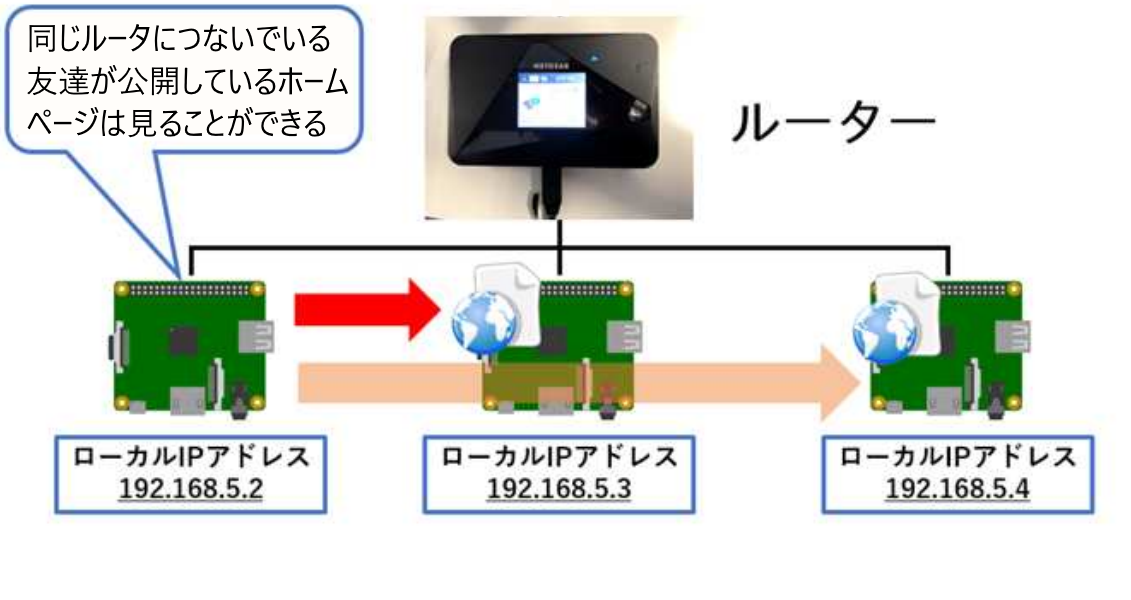
\includegraphics[width=100mm]{./slide07-img/slide07-img015.png}}
        \end{minipage}
\end{frame}

\begin{frame}[fragile]
	\frametitle{HTMLを復習しよう\\テキスト P.\pageref{1:P:HTML}-.\pageref{1:P:HP}~~~\raisebox{-3mm}{
\includegraphics[width=0.06\textwidth]{./slide07-img/raspberry.png}}}
      \large\textbf{教科書をよみながら、問題をやってみよう}
				\begin{itemize}\small
					\item \ref*{1:E:HTML} :P.\pageref{1:E:HTML}
					\item \ref*{1:Q:HTML} :P.\pageref{1:Q:HTML}
				\end{itemize}
      \vfill
      \large\textbf{わからないことは、放っておかず、すぐに TA に聞きましょう}
\end{frame}

\begin{frame}[fragile]
	\frametitle{ウェブサーバを立ち上げよう\\テキスト P.\pageref{1:P:HP}~~~\raisebox{-3mm}{
\includegraphics[width=0.06\textwidth]{./slide07-img/raspberry.png}}}
    \textbf{クライアントとサーバについて知ろう}\\
			\begin{minipage}{\textwidth}
                {\upshape
                  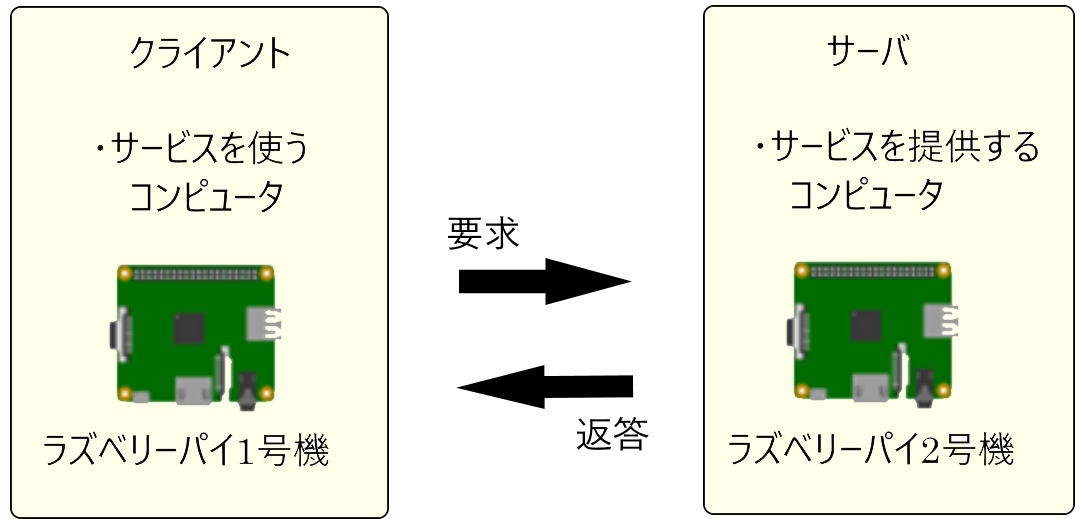
\includegraphics[width=\textwidth]{./slide07-img/slide07-img014.png}}
            \end{minipage}
            \begin{itemize}\small
                \item クライアントとサーバーは同じコンピュータにあっても問題ありません。
            \end{itemize}
\end{frame}

\begin{frame}[fragile]
	\frametitle{ウェブサーバを立ち上げよう\\テキスト P.\pageref{1:P:HP}~~~\raisebox{-3mm}{
\includegraphics[width=0.06\textwidth]{./slide07-img/raspberry.png}}}
            \begin{itemize}\small 
                \item 違うルータに接続している子のIPアドレスを入力しても、アクセスすることはできません。
            \end{itemize}
			\begin{minipage}{\textwidth}
                {\upshape
                  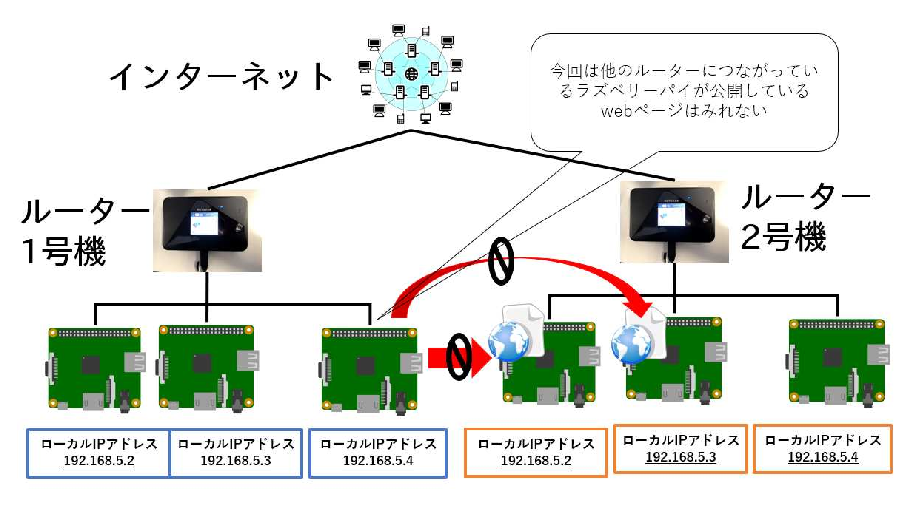
\includegraphics[width=\textwidth]{text07-img/ome7-img045}}
            \end{minipage}
\end{frame}

\begin{frame}[fragile]
	\frametitle{ウェブサーバを立ち上げよう\\テキスト P.\pageref{1:P:HP}-P.\pageref{1:P:CGI}~~~\raisebox{-3mm}{
\includegraphics[width=0.06\textwidth]{./slide07-img/raspberry.png}}}
      \large\textbf{教科書をよみながら、問題をやってみよう}
				\begin{itemize}\small
					\item \ref*{1:E:myHP} :P.\pageref{1:E:myHP}
					\item \ref*{1:friend} :P.\pageref{1:friend}
					\item \ref*{1:Q:otherHP} :P.\pageref{1:Q:otherHP}
				\end{itemize}
      \vfill
      \large\textbf{わからないことは、放っておかず、すぐに TA に聞きましょう}
\end{frame}
